\chapter{\iflanguage{ngerman}{Übersicht Hybrider OP-Saal}{Overview}}
\label{sec:overview}

Weniger invasive Eingriffe, geringeres Risiko und kürzere Operations-und Krankenhausaufenthalte sind Anforderungen die heutzutage an Ärzte und Operationssäle gestellt werden \cite{DerDigitaleOperationssaal}. Anforderungen, welchen ein konventioneller OP-Saal nicht mehr gerecht werden kann. Aus diesem Grund findet ein Umstieg zum Hybriden/ Digitalen/ Multifunktionalen oder auch Hochpräzisions OP-Saal statt. Unabhängig der Bezeichnung, geht es darum den OP-Saal zu digitalisieren und Bildgebende Verfahren wie Röntgen oder Ultraschall während der Operation einzusetzen.

In den folgenden Kapiteln wird immer vom Hybriden OP-Saal die Rede sein und es werden die Unterschiede vom Hybriden zum Konventionellen OP-Saal herausgearbeitet, sowie in welchen Einsatzgebieten der Hybride OP-Saal bereits verwendet wird und welche Vorteile dieser mit sich bringt.

\subsection{Hybrider OP-Saal vs. Konventioneller OP-Saal} 

\begin{figure} [H]
	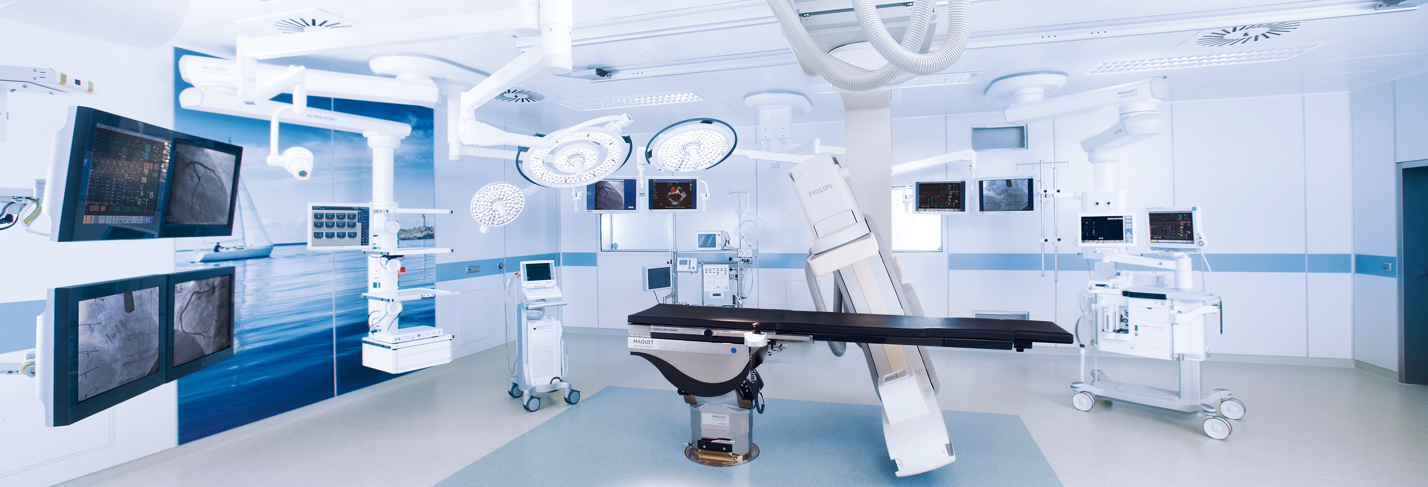
\includegraphics[scale = .3]{Content/Pictures/hybrid-or.png}
	\caption{Hybrider OP-Saal von Maquet mit einem an der Decke fixierten C-Bogen \cite{Maquet}.}
	\label{fig:hybridor}
\end{figure}

Ein Hybrider OP-Saal (Beispiel in Abb. \ref{fig:hybridor}) ist die Kombination aus einem sterilen konventionellen OP-Saal mit qualitativ hochwertiger Bildgebung. Hinzu kommt ein multifunktionalen OP-Tisch, digitale Datenregistrierung und Dokumentation sowie ungehinderter Datenaustausch innerhalb und außerhalb des OPs. Zur Steuerung und Kontrolle der Geräte und Systeme im OP-Saal steht ein Interface zur Verfügung \cite{HybriderVsKonventioneller,KarlStorz}. Darüber hinaus ist ein Hybrider OP-Saal, gegenüber einem Konventionellen OP-Saal, ein fachbereichsübergreifender chirurgischer Arbeitsbereich. Er wird gleichermaßen von der Neurochirurgie, Gefäßchirurgie, Onkologie, Kardiologie, Unfallchirurgie und vielen weiteren Bereichen genutzt \cite{Getinge}.\\
Mobile C-Bogen sowie Ultraschall- und Endoskopiegeräte gehören zur Standardausrüstung in Konventionellen OP-Sälen \cite{TechnicalConsiderations}. Für komplexe Operationsvorgänge wie bspw. bei Transkathetertechniken und für die Visualisierung der dünnen Führungsdrähte, wird jedoch eine leistungsstärkere Ausrüstung benötigt. Aus diesem Grund werden die mobilen C-Bogen durch befestigte ersetzt. Zur ergänzenden Ausrüstung des Hybriden OP-Saals können noch weitere Geräte für die intraoperative Bildgebung, wie Computertomographen (CT), Magnetresonanztomographen (MRT) oder Angiografieanlagen gehören \cite{OPderZukunft}. 
Die befestigten C-Bogen ermöglichen qualitativ hochwertige Echtzeitbildgebung mit Fluroskopie (Abb. \ref{fig:fluroscopy}) mit deren Hilfe Katheter durch den Körper geführt werden können. Ein Weiteres Verfahren ist die Digitale Subtraktionsangiographie (Abb. \ref{fig:dsa}). Dabei werden zwei Bilder vom jeweilig abzubildenden Gebiet, einmal mit und einmal ohne Kontrastmittel, angefertigt. Bei Subtraktion der beiden Bilder bleiben die Blutgefäße mit dem Kontrastmittel zurück \cite{CurrentAndFuture}. Darüber hinaus bieten MRT und CT die Möglichkeit hochauflösende Bilder von Geweben und Organen anzufertigen (Abb. \ref{fig:mrtct}).\\

\begin{figure}[!htb]
	\minipage{0.32\textwidth}
	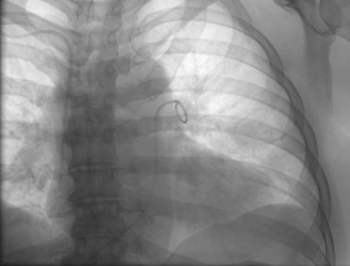
\includegraphics[width=\linewidth]{Content/Pictures/fluroscopy.png}
	\caption{Fluroskopie Aufnahme durch einen C-Bogen \cite{CurrentAndFuture}.}
	\label{fig:fluroscopy}
	\endminipage\hfill
	\minipage{0.32\textwidth}
	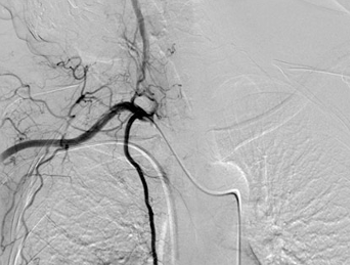
\includegraphics[width=\linewidth]{Content/Pictures/dsa.png}
	\caption{2D Bild mit Digitaler Subtraktionsangiographie (DSA) \cite{CurrentAndFuture}.}
	\label{fig:dsa}
	\endminipage\hfill
	\minipage{0.32\textwidth}%
	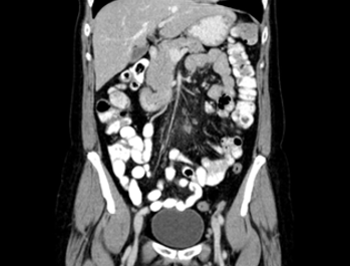
\includegraphics[width=\linewidth]{Content/Pictures/mrtct.png}
	\caption{CT-Aufnahme des Magens und Zwölffingerdarms \cite{CTBild}.}
	\label{fig:mrtct}
	\endminipage
\end{figure}

Somit können während eines Operationsvorgangs Diagnose und Therapiekontrolle vorgenommen, sowie minimal invasive Behandlungsverfahren durchgeführt werden \cite{SHG-Kliniken}. Auch ist es möglich \glqq während der Operation - und nicht erst danach - Bildkontrollen durch[zu]führen und allenfalls Korrekturmaßnahmen [zu] ergreifen\grqq{} \cite{OPderZukunft}. 

\subsection{Vorteile und wichtige Einsatzgebiete}

Wie Hybride OP-Säle Operationsvorgänge unterstützen, soll in der Neurochirurgie anhand der Kompensation des Brain Shifts, in der Gefäßchirurgie anhand des Setzens von Prothesen bei Aortenaneurysmen und in der Onkologie anhand der Tumorentfernung, erklärt werden.

\textbf{Neurochirurgie:}
Das Gehirn ist eine komplexe dreidimensionale Struktur, bei der sogenannte Brain Shifts (Verschiebungen der Gehirnstruktur Abb. \ref{fig:brainshift}) während einer Operation auftreten können. Ursachen für Brain Shifts können die Entfernung oder das Anschwellen von Gewebe, sowie der Verlust von Hirnwasser sein. Kommt es während einer Operation zu den oben genannten Verschiebungen, dann stimmen die vor einer Operation angefertigten CT- oder MR-Bilder der Gehirnstruktur nicht mehr mit der aktuellen Struktur überein. Bild geführte neurochirurgische Systeme (Image Guided Neurosurgical Systems, kurz IGNS), die während der Operation als Navigationshilfe dienen, können wegen den inkorrekten Bilddaten nur noch begrenzt arbeiten \cite{BrainShiftInTumorResection}.\\
Intraoperativer Ultraschall (iUS) oder intraoperative MR-Bilder (iMR) können diesem Problem entgegenwirken und die fehlenden Informationen ergänzen, sodass das IGNS wieder einsetzbar ist. IMR ermöglicht, während der Operation regelmäßig hochauflösende Bilder von der Gewebestruktur des Gehirns anzufertigen. Im Falle eines Brain Shifts kann dann entsprechend reagiert werden. Auch bei anderen neurochirurgischen Anwendungen wie der Hirnbiopsie, Entfernung von Tumoren oder der Drainage von Zysten kann iMR von Vorteil sein \cite{BrainShiftInTumorResection}.\\
Obwohl iMR als verlässlichste Option gilt, Bilder vom Gehirn anzufertigen und Brain Shifts zu erkennen, hat iUS den Vorteil kostengünstig Echtzeitzeitbilder zu produzieren. Die Kombination aus einem präoperativen MR-Bild und iUS reicht aus, um Gewebeveränderungen zu registrieren und die Korrektheit des IGNSs zu beurteilen. Im Gegensatz zu iMR, mit einer Bildaufnahmezeit von 15 Minuten, kann ein iUS-Bild in 5 Minuten aufgenommen werden. Aufgrund der vergleichbar schlechten Bildqualität gegenüber iMR wird iUS bisher begrenzt in der Neurochirurgie verwendet. Neue Ansätze (siehe Kapitel 4.1) ermöglichen jedoch die Möglichkeit einer genaueren US-Bildgebung für diesen Bereich \cite{BrainShiftInTumorResection}.

\begin{figure}[!htb]
	\minipage{0.45\textwidth}
	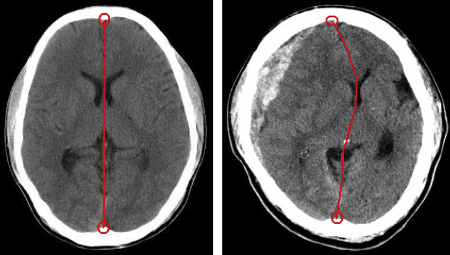
\includegraphics[width=\linewidth]{Content/Pictures/brainshift.png}
	\caption{(links) Keine Verschiebung, (rechts) Verschiebung der Mittellinie des Gehirns (midline brain shift) durch Anschwellen von Gewebe \cite{BrainShiftImage}.}
	\label{fig:brainshift}
	\endminipage\hfill
	\minipage{0.45\textwidth}%
	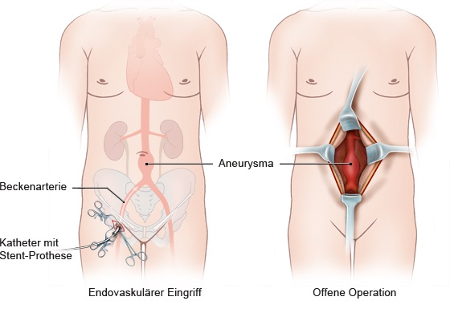
\includegraphics[width=\linewidth]{Content/Pictures/bauchaorten.png}
	\caption{(links) Endovaskulärer Eingriff bei einem Bauchaortenaneurysma mit Stent-Prothese gegenüber (rechts) einer offenen Operation mit normalen Prothesen \cite{BauaortenaneurysmaBild}.}
	\label{fig:bauchaorten}
	\endminipage
\end{figure}

\textbf{Gefäßchirurgie:}
Die Gefäßchirurgie profitiert von Hybriden OP-Sälen durch intraoperative Echtzeitbildgebung. Diese erlaubt den Fortschritt eines Katheters durch die Gefäße zu beobachten. Dadurch können das Ergebnis, wie das Setzen und richtige Sitzen einer Prothese, beurteilt werden \cite{DresdnerUniklinikum,TickendeBombeImBauch}. In Bezug auf ein Aortenaneurysma, eine krankhafte Erweiterung der Hauptschlagader, ergeben sich alternative Möglichkeiten der Operationsdurchführung. Da Aortenaneurysmen ruptieren und zu lebensbedrohlichen Blutungen führen können, muss ab einem gewissen Durchmesser der Erweiterung eine Prothese gesetzt werden \cite{Aortenaneurysma}. Die Operation kann entweder als offene Operation mit konventionellen Prothesen durchgeführt werden oder mit einem schonenden Verfahren und Implantation großer maßgefertigter Gefäßprothesen im Hybriden OP-Saal (siehe Abb. \ref{fig:bauchaorten}) \cite{DresdnerUniklinikum}. \\
Die offene Operation, bei der bei Bauchaneurysmen ein großer Schnitt in die Bauchdecke gemacht werden muss, weist gute Langzeitergebnisse auf, ist aber belastet und mit vergleichsweise langen Erholungszeiten verbunden \cite{TickendeBombeImBauch}. Da Aortenaneurysmen verstärkt im höheren Alter (> 60 Jahre) auftreten, kommt für diese Patienten eine offene Operation nicht mehr in Frage \cite{Aortenaneurysma}. \\
Alternativ wird deshalb beim schonenden Verfahren vor der Operation ein CT Bild angefertigt, welches dann mit den während der Operation entstehenden zwei- oder dreidimensionalen Bildern der Röntgenkontrolle kombiniert wird. Dies ermöglicht eine Stent-Prothese minimalinvasiv einzusetzen. Mithilfe eines Katheters kann dabei über einen kleinen Zugang in der Leiste durch das abgebildete Gefäß navigiert werden. Eine zusätzliche Software zur Navigationshilfe trägt dazu bei, die Prothese durch die Gefäße ans Ziel zu bringen \cite{DresdnerUniklinikum,TickendeBombeImBauch}.

\textbf{Onkologie:}
In der Onkologie hat man im Hybriden OP-Saal den Vorteil, dass nachdem ein Tumor entfernt und bevor die Operation abgeschlossen wurde, ein Kernspin mit dem MRT gemacht werden kann. Ohne den Patienten zu transportieren kann sichergestellt werden, dass tatsächlich keine Rückstände des Tumors übersehen wurden. Sollte dem nicht der Fall sein, kann direkt nachkorrigiert werden. Durch diese Korrekturmöglichkeit können Folgeoperationen erspart bleiben \cite{AerzteZeitung}. In mehr als einem drittel der Fälle, in denen die vollständige Entfernung eines Tumors angenommen wurde, wurden mit iMR noch Rückstände festgestellt und nachkorrigiert \cite{BrainShiftInTumorResection}.

\textbf{Fazit:} Zusammenfassend ermöglicht der Hybride OP-Säle präziseres, sicheres und schonenderes operieren durch minimalinvasive Eingriffe, welche weniger belastend für den Patienten sind \cite{DresdnerUniklinikum}. Das wiederum  führt zu kürzeren Krankenhausaufenthalten und zu Kosteneinsparungen in der Nachbetreuung und -behandlung. Der beliebig positionierbare OP-Tisch in Kombination mit dem hochbeweglichen C-Bogen sorgen für bestmögliche Röntgenbildaufnahmen. Diese können zur Unterstützung vor, während und nach der Operation eingesetzt werden \cite{DresdnerUniklinikum}. Entscheidungen über den Fortlauf der Operation können so besser getroffen werden, Ergebnisse beurteilt und gegebenenfalls nachkorrigiert werden.

